\documentclass[a4paper, 12pt]{book}
\usepackage[spanish,es-tabla]{babel}
\usepackage[utf8]{inputenc}

\usepackage[left = 35mm, right = 25mm, top = 25mm, height = 206mm]{geometry}
\usepackage{fancyhdr}
\usepackage{graphicx}
\usepackage{lipsum}
\usepackage[square,numbers]{natbib}
\usepackage[skip=12pt,font=small]{caption}  %Tamaño de la leyenda
\usepackage{subcaption}
\usepackage{amsmath}
\usepackage{afterpage}
\usepackage{titlesec}
\usepackage{color, colortbl}
\usepackage{listings}
\usepackage{xcolor}
\usepackage{float}
\usepackage{eurosym}
\usepackage{enumitem}
\usepackage{amssymb}
\usepackage{array}
\usepackage{wrapfig}
\usepackage{multirow}
\usepackage{tabularx}
\usepackage{url}
\usepackage{eurosym}
\usepackage{appendix}
\usepackage{pdfpages}
\usepackage{pdflscape} %poner pdf horizontal
\usepackage[hidelinks]{hyperref}%para el hiperlink de las secciones
\usepackage[newfloat]{minted}
\usepackage[nottoc]{tocbibind}
\usepackage{glossaries}


\usepackage{tikz} % Diagramas de flujo
\usetikzlibrary{shapes.geometric, arrows} %Libería de flechas

\usepackage{datetime}
\newdateformat{monthyeardate}{\monthname, \THEYEAR}

% Entorno para código
\newenvironment{code}{\captionsetup{type=listing}}{}

% Cambiamos el caption de los listing a español
\renewcommand{\listingname}{Código}

 % Cambiamos el idioma del índice de códigos
\renewcommand*{\listlistingname}{Índice de Códigos}

\newfloat{diagrama}{htbp}{loc}
\floatname{diagrama}{Diagrama}
\newcommand{\listofdiagrams}{\listof{diagrama}{Índice de Diagramas de Flujo}}
\floatstyle{plaintop}
\restylefloat{table}

\graphicspath{ {Imagenes/} }


\definecolor{codegreen}{rgb}{0,0.6,0}
\definecolor{codegray}{rgb}{0.5,0.5,0.5}
\definecolor{codepurple}{rgb}{0.58,0,0.82}
\definecolor{backcolour}{rgb}{0.95,0.95,0.92}
\definecolor{LightCyan}{rgb}{0.88,1,1}
\lstdefinestyle{codestyle}{
    backgroundcolor=\color{backcolour},
    commentstyle=\color{codegreen},
    keywordstyle=\color{magenta},
    numberstyle=\tiny\color{codegray},
    stringstyle=\color{codepurple},
    basicstyle=\ttfamily\footnotesize,
    breakatwhitespace=false,
    breaklines=true,
    captionpos=b,
    keepspaces=true,
    %numbers=left,
    %numbersep=5pt,
    showspaces=false,
    showstringspaces=false,
    showtabs=false,
    tabsize=2,
    literate=
    {á}{{\'a}}1 {é}{{\'e}}1 {í}{{\'i}}1 {ó}{{\'o}}1 {ú}{{\'u}}1
    {Á}{{\'A}}1 {É}{{\'E}}1 {Í}{{\'I}}1 {Ó}{{\'O}}1 {Ú}{{\'U}}1
    {à}{{\`a}}1 {è}{{\`e}}1 {ì}{{\`i}}1 {ò}{{\`o}}1 {ù}{{\`u}}1
    {À}{{\`A}}1 {È}{{\'E}}1 {Ì}{{\`I}}1 {Ò}{{\`O}}1 {Ù}{{\`U}}1
    {ä}{{\"a}}1 {ë}{{\"e}}1 {ï}{{\"i}}1 {ö}{{\"o}}1 {ü}{{\"u}}1
    {Ä}{{\"A}}1 {Ë}{{\"E}}1 {Ï}{{\"I}}1 {Ö}{{\"O}}1 {Ü}{{\"U}}1
    {â}{{\^a}}1 {ê}{{\^e}}1 {î}{{\^i}}1 {ô}{{\^o}}1 {û}{{\^u}}1
    {Â}{{\^A}}1 {Ê}{{\^E}}1 {Î}{{\^I}}1 {Ô}{{\^O}}1 {Û}{{\^U}}1
    {œ}{{\oe}}1 {Œ}{{\OE}}1 {æ}{{\ae}}1 {Æ}{{\AE}}1 {ß}{{\ss}}1
    {ç}{{\c c}}1 {Ç}{{\c C}}1 {ø}{{\o}}1 {å}{{\r a}}1 {Å}{{\r A}}1
    {€}{{\EUR}}1 {£}{{\pounds}}1 {ñ}{{\~{n}}}1
}

\tikzstyle{startstop} = [rectangle, rounded corners, 
minimum width=3cm, 
minimum height=1cm,
text centered, 
draw=black, 
fill=red!30]

\tikzstyle{io} = [trapezium, 
trapezium stretches=true, % A later addition
trapezium left angle=70, 
trapezium right angle=110, 
minimum width=3cm, 
minimum height=1cm, text centered, 
draw=black, fill=blue!30]

\tikzstyle{process} = [rectangle, 
minimum width=3cm, 
minimum height=1cm, 
text centered, 
text width=3cm, 
draw=black, 
fill=orange!30]

\tikzstyle{decision} = [diamond, 
minimum width=3cm, 
minimum height=1cm, 
text centered, 
draw=black, 
fill=green!30]
\tikzstyle{arrow} = [thick,->,>=stealth]
%----------------------------------------------------------------------------------------
%	ENCABEZADOS Y PIE DE PAGINA
%----------------------------------------------------------------------------------------

\pagestyle{fancy}
	\fancypagestyle{cuerpo}{
		\fancyfoot{}
		\fancyfoot[L]{Trabajo Fin de Grado} %Autor
		\fancyfoot[C]{}
		\fancyfoot[R]{- \thepage \ -}
		\fancyhead{}
		\fancyhead[L]{\leftmark} %Nombre del documento
		\fancyhead[R]{
\includegraphics[height=1.8cm]{logo_uco}} %Logo Universidad
		\renewcommand{\headrulewidth}{0.4pt}
		\renewcommand{\footrulewidth}{0.4pt}
		\setlength{\headheight}{65pt}
	}
	\fancypagestyle{indice}{
		\fancyfoot{}
		\fancyfoot[L]{\AutorTFG} %Autor
		\fancyfoot[R]{- \thepage \ -} %Asignatura
		\fancyhead{}
		\fancyhead[L]{Trabajo Fin de Grado} %Nombre del documento
		\fancyhead[R]{
\includegraphics[height=1.8cm]{logo_uco}} %Logo
		\renewcommand{\headrulewidth}{0.4pt}
		\renewcommand{\footrulewidth}{0.4pt}
		\setlength{\headheight}{65pt}
	}

	\fancypagestyle{plain}{% % <-- this is new
		\fancyfoot{}
		\fancyfoot[L]{Trabajo Fin de Grado} %Autor
		\fancyfoot[C]{} %ecc
		\fancyfoot[R]{- \thepage \ -}
		\fancyhead{}
		\fancyhead[L]{\leftmark} %Nombre del documento
		\fancyhead[R]{
\includegraphics[height=1.8cm]{logo_uco}} %Logo Universidad
		\renewcommand{\headrulewidth}{0.4pt}
		\renewcommand{\footrulewidth}{0.4pt}
		\setlength{\headheight}{65pt}
	}

\setcounter{secnumdepth}{4}

\pagenumbering{empty}


%%%%%%%%%
% ANEXO %
%%%%%%%%%

% Para que ponga ANEXO en vez de APENDICE
 \addto\captionsspanish{\renewcommand{\appendixname}{Anexo}} %para que ponga anexo y no apéndice.

\makeglossaries
\raggedbottom  % Quita huecos grandes en blanco
\begin{document}

%%%%%%%%%%%
% PORTADA %
%%%%%%%%%%%
\newcommand{\TituloTFG}{Estudio comparativo de métodos de aprendizaje automático en la detección de malware}
\newcommand{\AutorTFG}{Manuel Jesús Mariscal Romero}
\newcommand{\DirectorUno}{D. David Guijo Rubio}
\newcommand{\DirectorDos}{D. Víctor Manuel Vargas Yun}
\newcommand{\Grado}{Grado en Ingeniería Informática}



% Definición de colores usados en la portada
\definecolor{epsc:oscuro}{HTML}{280091}
\definecolor{epsc:medio}{HTML}{4C5CC5}
\definecolor{epsc:verde}{HTML}{00B299}
\definecolor{epsc:claro}{HTML}{3FCFD5}

\definecolor{PORTADA_0}{cmyk}{1.00,0.00,0.07,0.28,1.00}

\definecolor{PORTADA_1}{cmyk}{0.58,0.55,0.00,0.44,1.00}

\definecolor{friendlyGray}{HTML}{f0f0f0}

\thispagestyle{empty}

\begin{tikzpicture}[remember picture, overlay]
  % Top
  \node [anchor=north east, inner sep=0pt]  at (current page.north east)%
    {
\includegraphics[height=6cm]{Portada/Img/topRightCorner.pdf}};
  % Bottom
  \node [anchor=south west, inner sep=0pt]  at (current page.south west)%
    {
\includegraphics[height=6cm]{Portada/Img/bottomLeftCorner.pdf}};
  \node (uco) [anchor=south east, inner sep=0pt, xshift=-10mm, yshift=10mm]  at (current page.south east)%
    {
\includegraphics[height=2cm]{Portada/Img/uco_escudo}};
  \node [anchor=south east, inner sep=0pt, xshift=-10mm]  at (uco.south west)%
    {
\includegraphics[height=2cm]{Portada/Img/emblema-ing-industrial.pdf}};
    %{
\includegraphics[height=2cm]{Portada/Img/emblema-ing-informatica.png}};
\end{tikzpicture}

% Título del trabajo, autor y directores
\begin{center}
\vspace*{2cm}
\vfill
\vfill
\vfill
\vfill

\includegraphics[width=12.5cm]{Portada/Img/LogotipoEPSC}
\vfill
\vfill

{\color{epsc:verde}
\large

\textbf{TRABAJO FIN DE GRADO}

\textit{\Grado}
} \vspace{1mm}

{\color{epsc:oscuro}

\textbf{\large \TituloTFG}

\vspace{14.35mm}
\begin{tabular}{rl}
\textbf{Autor:} & \AutorTFG\\
\textbf{Directores:} & \DirectorUno\\
                     & \DirectorDos\\
\end{tabular}

\vspace{6.79mm}
\textbf{\monthyeardate{\today}}        % Fecha de compilación en formato mes, año

}
\end{center}
\endinput

\newpage
\thispagestyle{empty}   % Página en blanco entre la portada y el comienzo del documento
\mbox{}
$\ $
\thispagestyle{empty} % para que no se numere esta pagina
\newpage
$\ $
\thispagestyle{empty} % para que no se numere esta pagina

%%%%%%%%%%%%%%%
% DEDICATORIA %
%%%%%%%%%%%%%%%
\pagenumbering{Roman} % para comenzar la numeracion de paginas en numeros romanos
% \pagestyle{indice}
% \thispagestyle{indice}
% \begin{flushright}
% \textit{Dedicado a \\
% mi familia}
% \end{flushright}

%%%%%%%%%%%%%%%%%%%
% AGRADECIMIENTOS %
%%%%%%%%%%%%%%%%%%%
% \chapter*{Agradecimientos}

\addcontentsline{toc}{chapter}{Agradecimientos} % si queremos que aparezca en el índice

\markboth{Agradecimientos}{Agradecimientos} % encabezado

RELLENAR



%%%%%%%%%%%%%%%%%%%%%%
% RESUMEN Y ABSTRACT %
%%%%%%%%%%%%%%%%%%%%%%
\chapter*{Resumen}
\addcontentsline{toc}{chapter}{Resumen} % si queremos que aparezca en el índice
\markboth{Resumen}{Resumen} % encabezado

Este proyecto se centra en la aplicación de técnicas de aprendizaje automático para la detección de \textit{malware}. El objetivo principal es comparar distintos algoritmos, tanto los estudiados en el plan de estudios de Ingeniería Informática como otros que no forman parte de la formación académica, con el fin de determinar cuáles se adaptan mejor a este problema.

\vspace{1em}

Para ello, se utilizan bases de datos públicas de \textit{malware}, adaptadas mediante técnicas de preprocesamiento, balanceo y reducción de la dimensionalidad. Posteriormente, se implementa un protocolo experimental que incluye la optimización de hiperparámetros, la validación cruzada estratificada y la repetición de experimentos con diferentes semillas para garantizar la reproducibilidad.

\vspace{1em}

Finalmente, se analizan los resultados obtenidos en términos de precisión, eficiencia y viabilidad computacional, destacando las ventajas e inconvenientes de cada enfoque y aportando una visión comparativa que pueda servir de referencia para futuros estudios en la detección automática de \textit{malware}.

\vspace{2em}

\textbf{Palabras clave:} Aprendizaje automático, Detección de \textit{malware}, Clasificación, Ciberseguridad

\chapter*{Abstract}
\addcontentsline{toc}{chapter}{Abstract} % si queremos que aparezca en el índice
\markboth{Abstract}{Abstract} % encabezado

This project focusses on the application of machine learning techniques for malware detection. The main objective is to compare different algorithms, both those studied in the Computer Engineering curriculum and others not included in the formal academic training, to determine which are better suited to this problem.

\vspace{1em}

For this purpose, public malware datasets are used, adapted through preprocessing, data balancing and dimensionality reduction techniques. Afterwards, an experimental protocol including hyperparameter optimization, stratified cross-validation and the repetition of experiments with different random seeds, is implemented to guarantee reproducibility.

\vspace{1em}

Finally, the results are analyzed in terms of accuracy, efficiency and computational viability, with special focus on the advantages and disadvantages of each approach and providing a comparative perspective to serve as a reference for future research on automated malware detection.

\vspace{2em}

\textbf{Keywords:} Machine Learnig, Malware detection, Clasification, Cibersecurity.

%%%%%%%%%%%%%%%%%%
% INDICE GENERAL %
%%%%%%%%%%%%%%%%%%
\newpage
\thispagestyle{fancy}

\tableofcontents

\cleardoublepage
\listoffigures

\cleardoublepage
\listoftables

% Descomentar las siguientes líneas si tienes pensado añadir diagramas de flujo.
% \cleardoublepage
% \phantomsection
% \addcontentsline{toc}{chapter}{Índice de diagramas de flujo}
% \listofdiagrams

\cleardoublepage
%\phantomsection
\addcontentsline{toc}{chapter}{Lista de Acrónimos}


\newacronym{iot}{IoT}{Internet of Things}


\printglossary[type=\acronymtype, title={Acrónimos}]

%---------------------%
%	CUERPO DE TEXTO   %
%---------------------%

\afterpage{\null\newpage}

\newpage
\newpage

\pagestyle{cuerpo}
\thispagestyle{cuerpo}

\pagenumbering{arabic}

%%%%%%%%%%%%%%%%%%%%%%%%%%%%%%%%%%%%%%%%%%%%%%%%%%%%%%%%%%%%%%%%%%%%%
%                         ESTRUCTURA CONTENIDO                      %
%%%%%%%%%%%%%%%%%%%%%%%%%%%%%%%%%%%%%%%%%%%%%%%%%%%%%%%%%%%%%%%%%%%%%

%------------------%
%	CAPÍTULOS      %
%------------------%

\chapter{Introducción}
\label{ch:introduccion}



\chapter{Estado de la técnica}
\label{ch:estado_tecnica}

En este capítulo se presentan los fundamentos teóricos más relevantes que sirven como base para el desarrollo de este proyecto. Se revisan conceptos clave relacionados con el aprendizaje automático y su aplicación en la detección de \textit{malware}, así como las nociones generales de ciberseguridad y los enfoques más utilizados en la identificación de software malicioso.

\section{Aprendizaje automático}
\label{sec:aprend_auto}

El aprendizaje automático se puede entender como <<la creación de algoritmos y modelos que permiten a los ordenadores aprender y hacer predicciones sin ser específicamente programados>> \cite{mwclass}.

\vspace{1em}

Inicialmente, los cálculos estadísticos se resolvían con máquinas electromecánicas, como la máquina tabuladora, desarrollada en 1890 por Herman Hollerith \cite{maquina_tabuladora}. Años más tarde, se presentó la neurona de McCulloch-Pitts, el primer modelo matemático de una neurona biológica, considerado por muchos como el punto de partida para el aprendizaje automático y la base de importantes modelos de cálculo \cite{inproceedings}. Hoy en día, el aprendizaje automático es esencial en diferentes ámbitos, como la investigación o los negocios, y emplea algoritmos avanzados capaces de hacer predicciones muy precisas sobre datos desconocidos.

\vspace{1em}

Los algoritmos desarrollados se pueden dividir en aprendizaje supervisado, no supervisado, semisupervisado y por refuerzo, entre otros. A su vez, y de manera independiente a la clasificación anterior, se pueden dividir en técnicas de clasificación y regresión, siendo las primeros las que nos ocupan en este proyecto. Algunas de las principales técnicas de clasificación ordinal son: árboles de decisión, redes neuronales artificiales, máquinas de vectores de soporte (SVM, por sus siglas en inglés) y algoritmos de agrupamiento.

\vspace{1em}

Todas estas técnicas se pueden adaptar a las necesidades actuales de la ciberseguridad. Los tipos de ataques, \textit{malware} o vulnerabilidades de los sistemas se están haciendo cada vez más frecuentes, no solo aumentando en cantidad, sino también en complejidad. Estos algoritmos pueden predecir si un \textit{software} es malicioso, si tiene vulnerabilidades o si un correo electrónico puede considerarse un intento de \textit{phishing}.

\vspace{1em}

A continuación se comentarán algunas de las principales técnicas y modelos que podrían llegar a aplicarse en este estudio si fuera necesario.

\subsection{Balanceo de datos}
\label{subsec:balanceo}

Es muy habitual que los conjuntos de datos se encuentren desbalanceados. Esto significa que la cantidad de patrones pertenecientes a una o varias clases son significativamente menores a la clase mayoritaria. Por ejemplo, como veremos más adelante en la tabla \ref{tabla:codificacion_malware}, la clase de patrones no malicionsos representa aproximadamente la mitad del total de patrones, en torno a 150000 patrones, mientras que la clase exploit solo tiene 12 patrones \cite{balanceo}. Debido a este desbalanceo es probable que la capacidad de generalización del modelo se vea afectada.

\vspace{1em}

Para mitigar estos problemas, las dos principales técnicas son el sobremuestreo y el submuestreo, \textit{oversampling} y \textit{undersampling} por sus términos en inglés.

\subsubsection{Sobremuestreo}
\label{subsubsec:oversampling}

Las técnicas de sobremuestreo, \textit{oversampling} en inglés, buscan aumentar la representación de la clase minoritaria generando nuevas instancias a partir de los casos existentes. El problema que presenta esta técnica es el riesgo de introducir información no real \cite{resamplig}. Entre los métodos de \textit{oversampling} más destacados se encuentran:

\begin{enumerate}
	\item \textbf{\textit{Random oversampling.}} \\
		Es la técnica más sencilla, ya que copia los patrones de la clase minoritaria hasta alcanzar la cantidad deseada. Es habitual que se haga hasta igualar a la clase mayoritaria \cite{resamplig}.
	\item \textbf{\textit{Synthetic Minority Oversampling Technique (SMOTE).}.} \\
		Genera instancias sintéticas de la clase minoritaria en lugar de replicar ejemplos existentes. Para ello, selecciona un ejemplo de la clase minoritaria y crea nuevos puntos interpolando con sus vecinos más cercanos \cite{ELREEDY201932}.
	\item \textbf{\textit{Adaptative Synthetic Sampling (ADASYN).}} \\
		Es una extensión de SMOTE que genera más instancias sintéticas en las zonas donde la clase minoritaria es más difícil de aprender, es decir, donde está menos representada respecto a la mayoritaria \cite{ADASYN}.
\end{enumerate}

\subsubsection{Submuestreo}
\label{subsubsec:undersampling}

El \textit{undersampling} engloba las técnicas que tratan de igualar las distribuciones de datos desbalanceados eliminando muestras de la clase mayoritaria respetando la distribución de la clase minoritaria. Las soluciones a este problema pueden cambiar en función del algoritmo que decide los patrones a eliminar \cite{resamplig}. Las principales técnicas de \textit{undersampling} son:

\begin{enumerate}
	\item \textbf{\textit{Random undersampling.}} \\
		Es el método más sencillo, ya que solo se encarga de eliminar patrones de forma aleatoria de la clase mayoritaria. Lo habitual, y la técnica empleada en este estudio para la clasificación binaria, es igualar el número de patrones para cada clase. Su principal punto en contra es que puede eliminar datos útiles \cite{rundersampling}.
	\item \textbf{\textit{Condensed nearest neighbours}.} \\
		Es un algoritmo no paramétrico basado en instancias, donde la clasificación se determina a partir de los k casos más cercanos al punto. Es una técnica local que utiliza medidas de distancia para identificar la similitud entre observaciones \cite{cnn}.
	\item \textbf{\textit{Tomek links.}} \\
		Consiste en identificar pares de instancias pertenecientes a clases distintas que son mutuamente los vecinos más cercanos entre sí. Suelen encontrarse en las zonas de solapamiento entre clases y representan casos ruidosos. Se elimina del conjunto de datos la instancia perteneciente a la clase mayoritaria en cada par, reduciendo así el desbalanceo \cite{tomeklinks}.
	\item \textbf{\textit{Edited nearest neighbours.}} \\
		Consiste en revisar cada instancia del conjunto de datos y clasificarla según la regla de los k vecinos más cercanos. Si la instancia no coincide con la clase mayoritaria de sus vecinos, se considera ruidosa o mal ubicada y se elimina del conjunto \cite{enn}.
\end{enumerate}

\newpage
\subsection{Reducción de la dimensionalidad}
\label{subsec:red_dim}

En estadística, la reducción de la dimensionalidad es el proceso por el cual se reduce el número de variables aleatorias. Si aplicamos esto al aprendizaje automático, el objetivo a reducir es el número de características de cada patrón. Generalmente se aplica antes de la clasificación para evitar los efectos de la maldición de la dimensionalidad, que se ha comentado en la sección \ref{subsubsec:problemas}. La principal ventaja que aportan estas técnicas es reducir el tiempo de entrenamiento y la memoria utilizada en el mismo \cite{reddim}. A continuación, estudiaremos algunos de los principales métodos.

\begin{enumerate}
	\item \textbf{Análisis de componentes principales} \\
		El análisis de componentes principales se usa para describir un conjunto de datos en términos de nuevas características no correlacionadas, buscando la proyección donde los datos queden mejor representados según el método de mínimos cuadrados \cite{pca}.

	\item \textbf{Análisis factorial} \\
		Tiene el objetivo es identificar un conjunto reducido de factores latentes que explican la mayor parte de la varianza observada en los datos para descubrir las estructuras que generan las correlaciones entre las variables \cite{fa}.

	\item \textbf{Descomposición en valores singulares} \\
		Es una técnica algebraica que descompone una matriz en tres componentes: $U$, $\Sigma$ y $V^T$ \cite{dvs}.Esta descomposición permite representar los datos en un espacio reducido preservando la mayor parte de la información relevante.
\end{enumerate}

\subsection{Métricas de evaluación}
\label{subsec:2_metricas}

La elección de métricas de evaluación adecuadas es esencial para valorar de forma precisa el rendimiento de los modelos. No todas las métricas ofrecen la misma información. En esta sección se revisan las métricas más empleadas en la literatura especializada, destacando su utilidad, limitaciones y el tipo de información que aportan para la comparación de modelos.

\subsubsection{Exactitud}
\label{subsubsec:acc}

La exactitud o \textit{Accuracy} se corresponde con el porcentaje de aciertos que se han producido, es decir, los patrones clasificados correctamente respecto al total. Se calcula como la suma de verdaderos positivos (TP) y verdaderos negativos (TN) respecto al número total de patrones de entrada (N) \cite{metrics}.

\begin{equation}
	\label{eq:accuracy}
	\text{CCR} = \frac{TP+TN}{N}
\end{equation}

\subsubsection{Precisión}
\label{subsubsec:prec}

La precisión es una métrica que evalúa la proporción de patrones clasificados como positivas que realmente pertenecen a la clase positiva, es decir, mide como de confiable es el modelo cuando predice un positivo. Es muy relevante cuando el coste de clasificar erróneamente un negativo como positivo es alto.

\begin{equation}
	\text{Precisión} = \frac{TP}{TP + FP}
	\label{eq:precision}
\end{equation}

Donde \(TP\) representa el número de verdaderos positivos, y \(FP\) corresponde al número de falsos positivos.

\subsubsection{Sensibilidad}
\label{subsubsec:sens}

También conocida como exhaustividad o \textit{recall} en inglés, mide la capacidad del modelo para detectar correctamente los positivos de un conjunto de datos. Como se muestra en la ecuación \ref{eq:recall}, se calcula como la proporción entre el número de verdaderos positivos (TP) y la suma de verdaderos positivos y falsos negativos (FN) \cite{metrics}. Un valor alto de sensibilidad indica que se han obtenido pocos falsos negativos.

\begin{equation}
	\label{eq:recall}
	\text{Sensibilidad} = \frac{TP}{TP + FN}
\end{equation}

\subsubsection{Mínima sensibilidad}
\label{subsubsec:ms}

La mínima sensibilidad mide cómo de bien se clasifica la clase peor clasificada. Es útil en clasificación multiclase o con conjuntos de datos desbalanceados, ya que permite identificar si existe alguna clase que el modelo no está clasificando correctamente. Un valor alto indica que el modelo mantiene un buen rendimiento en todas las clases, mientras que un valor bajo revela que, al menos, una de ellas presenta un bajo grado de acierto. Si el modelo se deja una clase sin clasificar, el valor será 0.

\vspace{1em}

Sea \( S_i \) la sensibilidad de la clase \( i \), con \( n \) el número total de clases, la mínima sensibilidad se calcula como se muestra en la ecuación \ref{eq:ms}.

\begin{equation}
	MS = \min_{i \in \{1, 2, \dots, n\}} S_i
	\label{eq:ms}
\end{equation}

Donde la sensibilidad de cada clase \( S_i \) se obtiene mediante la ecuación \ref{eq:recall}

\newpage
\subsubsection{Valor-F}
\label{subsubsec:f1}

El valor-F o \textit{F1-score} mide el equilibrio entre la precisión y la sensibilidad \cite{metrics}. Se calcula como la media armónica entre ambas, lo que penaliza de forma más severa los valores extremos y proporciona una medida equilibrada del rendimiento del modelo. Es especialmente útil en problemas con clases desbalanceadas, ya que evita que un alto rendimiento en una sola métrica distorsione la evaluación global.

\subsubsection{Matriz de confusión}
\label{subsubsec:matrix}

Una matriz de confusión permite visualizar el rendimiento de un algoritmo de clasificación, normalmente supervisado. Cada fila representa las instancias en una clase real, mientras que cada columna representa las instancias en una clase predicha (o viceversa). La diagonal de la matriz representa las instancias correctamente clasificadas \cite{confmat}. Las matrices de confusión pueden utilizarse con cualquier algoritmo clasificador.

\subsection{Técnicas de validación}
\label{subsec:validacion}
% TODO: 



\subsubsection{Validación cruzada}
\label{subsubsec:cv}
% TODO: 



\subsubsection{Validación estratificada}
\label{subsubsec:ev}
% TODO: 



\subsubsection{Problemas de entrenamiento}
\label{subsubsec:problemas}
% TODO:  overfitting y underfitting, maldicion de la dimensionalidad

\subsection{Preprocesamiento de datos}
%\label{subsec:}
% TODO: 



\subsubsection{}
%\label{subsubsec:}
% TODO: 




\subsection{Algoritmos de clasificación}
%\label{subsec:}
% TODO: 

\subsubsection{Árboles de decisión}
\label{subsubsec:arboles}

% TODO: 

\subsubsection{\textit{Random forest}}
\label{subsubsec:randomforest}

% TODO: 

\subsubsection{\textit{K-NN}}
\label{subsubsec:kneighbors}

% TODO: 

\subsubsection{\textit{Ridge}}
\label{subsubsec:ridge}

% TODO: 

\subsubsection{Perceptrón multicapa}
\label{subsubsec:mlp}

% TODO: 

\subsubsection{Máquinas de vectores de soporte}
\label{subsubsec:svm}

% TODO: 

\subsubsection{\textit{Light Gradient-Boosting Machine}}
\label{subsubsec:lgbm}

% TODO: 

\section{Ciberseguridad}
\label{sec:ciberseguridad}

La ciberseguridad es la protección de la infraestructura informática y la información que hay en ella, abarcando \textit{software}, \textit{hardware} y redes. Para garantizar la seguridad, es esencial combinar estrategias de prevención con métodos de protección efectivos. Las estrategias de prevención, como el uso de \textit{firewalls}, \textit{software} antivirus actualizado y educación en ciberseguridad para los usuarios, se centra en identificar y mitigar posibles amenazas antes de que ocurran. Por otro lado, la protección se enfoca en responder a los incidentes y minimizar sus efectos, mediante herramientas como los sistemas de detección de intrusiones. Con esto, podemos llegar a la conclusión de que el objetivo de la seguridad es minimizar los riesgos de recibir un ataque y reducir el impacto en caso recibirlo \cite{ciberseguridad_def}. En esta sección nos centraremos en la ciberseguridad \textit{software}, concretamente en los aspectos relacionados con la detección y clasificación de malware.

\subsection{Conceptos generales}
\label{subsec:ciberseguridad_general}
% TODO: Breve introducción a la ciberseguridad, importancia en la sociedad digital, principales objetivos (confidencialidad, integridad, disponibilidad) y amenazas comunes.

\subsection{\textit{Malware}}
\label{subsec:malware}
% TODO: Definición de malware, evolución histórica, relevancia actual.

\subsubsection{Tipos de \textit{Malware}}
\label{subsubsec:tipos_malware}
El \textit{software} malicioso o \textit{malware} es cualquier tipo de \textit{software} que se introduce de manera encubierta con el objetivo de comprometer la confidencialidad, integridad o disponibilidad de la información o el sistema \cite{def_malware}. El \textit{malware} se ha convertido en una de las amenazas externas más relevantes debido al daño que puede llegar a causar en una organización. Podemos clasificar el \textit{malware} en diferentes categorías \cite{categoriamw} según su propósito:

\begin{itemize}
	\item Virus. Tienen como objetivo infectar archivos y sistemas informáticos. Se propagan cuando los usuarios comparten archivos o ejecutan programas infectados.
	\item Gusanos. Se propagan a través de las redes sin que tenga que intervenir el usuario.
	\item Troyanos. Se presentan como un \textit{software} legítimo. De esta forma intentan engañar al usuario para que lo descargue, instale y ejecute.
	\item \textit{Adware}. Muestra anuncios de forma intrusiva. Puede ser incrustada en una página web mediante gráficos, carteles, ventanas flotantes, o durante la instalación de algún programa al usuario, con el fin de generar lucro a sus autores.
	\item \textit{Spyware}. Trata de conseguir información de un equipo sin conocimiento ni consentimiento del usuario. Después transmite esta información a una entidad externa.
	\item \textit{Ransomware}. Conocido como secuestro de datos en español. Está diseñado para restringir el acceso a archivos o partes de un sistema y pedir un rescate para quitar la restricción.
	\item \textit{Rootkit}. Es un conjunto de \textit{software} que permite al atacante un acceso de privilegio a un ordenador, manteniendo presencia inicialmente oculta al control de los administradores.
	\item \textit{Keylogger}. Se encarga de registrar las pulsaciones que se realizan en el teclado, para memorizarlas en un fichero o enviarlas a través de Internet.
	\item \textit{Exploit}. Aprovecha un error o una vulnerabilidad de una aplicación o sistema para provocar un comportamiento involuntario.
	\item \textit{Backdoor}. Puerta trasera en español. Este tipo de \textit{software} permite un acceso no autorizado al sistema, evitando pasar por los métodos de autenticación.
\end{itemize}

\subsection{Técnicas de detección de \textit{Malware}}
\label{subsec:deteccion_malware}
% TODO: 

Ningún método de detección es infalible y los principales antivirus comerciales pueden combinar distintas técnicas en función de las necesidades. La detección basada en firmas siguen siendo el método más usado en términos absolutos porque son rápidas, eficientes y fáciles de implementar. Este método consiste en comparar archivos con una base de datos de patrones conocidos. Otros mecanismos son: la detección heurística, por comportamiento, \textit{sandbox} e inteligencia artificial \cite{antivirus}.

\vspace{1em}

Existen varias limitaciones de los métodos tradicionales frente a nuevas amenazas. Por ejemplo, para evadir la detección basada en firmas se generaba una cadena de bits única cada vez que se codificaba. Esto se denomina polimorfismo. Gracias a la heurística no era necesaria una coincidencia exacta con las firmas almacenadas, pero debido a la gran cantidad de variaciones que surgen a diario, su efectividad y la de otros mecanismos se ve comprometida \cite{limitaciones}. A continuación se estudiarán algunas de las técnicas más usadas.

\subsubsection{Detección basada en firmas}
\label{subsubsec:firmas}
% TODO: 

\subsubsection{Detección heurística y análisis estático}
\label{subsubsec:heuristica}
% TODO: 

\subsubsection{Detección basada en comportamiento (análisis dinámico)}
\label{subsubsec:comportamiento}
% TODO: 

\subsubsection{Métodos híbridos}
\label{subsubsec:hibridos}
% TODO: 

\subsubsection{Detección mediante aprendizaje automático}
\label{subsubsec:ml}
% TODO: Algoritmos de clasificación, extracción de características y métricas más usadas.


\subsection{Retos y tendencias}
\label{subsec:retos_tendencias}
% TODO: Limitaciones de las técnicas clásicas, evasión mediante ofuscación, necesidad de datasets representativos y uso creciente de IA y aprendizaje profundo en ciberseguridad.



\chapter{Formunación del problema}
\label{ch:formulacion_problema}
\chapter{Objetivos}
\label{ch:objetivos}

Debe de ser igual a los mencionados en el anteproyecto.

Describir el objetivo principal y los objetivos especificos llevados a cabo para conseguir el objetivo principal.

\chapter{Metodología de trabajo}
\label{ch:metodologia}

\section{Enfoque metodológico}

% TODO: Explica el tipo de estudio realizado (comparativo, experimental, descriptivo) y justifica por qué este enfoque es el más adecuado para los objetivos del proyecto. (experimental, descriptivo, comparativo, etc.).

\section{Procedimiento seguido}

% TODO: Detalla la secuencia de actividades, desde la recolección y preparación de datos hasta la obtención y análisis de resultados, especificando el orden lógico de ejecución.

\section{Técnicas y herramientas empleadas}

% TODO: Describe el software, librerías, lenguajes de programación y hardware utilizados, así como su función específica dentro del desarrollo del proyecto.

\section{Criterios de selección de datos y modelos.}

\subsection{Selección del conjunto de datos}
\label{subsec:select_dataset}

En lo que a \textit{malware} se refiere, \textit{BODMAS} \cite{bodmas} es uno de los conjuntos de datos más completos en la actualidad, con la ventaja para este proyecto de ya estar procesado y tener una amplia bibliografía. Otra opción interesante puede ser \textit{VirusShare} \cite{virusshare}, ya que cuenta con más de 99 millones de muestras de \textit{malware} actualizadas pero tiene varios inconvenientes para este proyecto. El primero, es que no incluye muestras de \textit{software} no malicioso y el segundo, que necesita un procesamiento previo para extraer las características. Todo esto conlleva un aumento de tiempo considerable para la realización del proyecto. Otra de las opciones estudiadas ha sido \textit{theZoo} \cite{thezoo}. En cuanto a este repositorio hemos podido observar que tiene los mismos inconvenientes que \textit{VirusShare} y no tiene sus ventajas. Por último tenemos \textit{Microsoft Malware Classification} \cite{malware-classification}. En este caso tenemos un conjunto de datos muy amplio con casi medio \textit{terabyte}, pero además de los inconvenientes ya comentados en los anteriores conjuntos, solo incluye \textit{malware} que afecta a equipos \textit{Windows}, lo que limitaría considerablemente el alcance del estudio.

\vspace{1em}

Teniendo en cuenta todo lo comentado hasta ahora sobre los distintos conjuntos de datos considerados, hemos decidido usar \textit{BODMAS}, ya que es el que mejor se adapta a las necesidades del estudio

\subsection{Selección de los modelos}
\label{subsec:select_model}



\chapter{Desarrollo y experimentación}
\label{ch:desarrollo}

En esta fase se lleva a cabo la implementación práctica del estudio, haciendo uso de los modelos de aprendizaje automático implementados principalmente en la biblioteca \textit{Scikit-Learn} de \textit{python}. Para ello se realiza un procesamiento de los datos, necesario para obtener un conjunto reducido y otro apto para la clasificación multiclase. Además, se configuran los entornos necesarios para su entrenamiento y evaluación, se establecen las métricas de rendimiento, los procedimientos de prueba y los escenarios de experimentación que permitirán obtener resultados consistentes y comparables. El objetivo es verificar, mediante pruebas controladas, la efectividad de cada método en la detección de \textit{malware}.

\vspace{1em}

La parte experimental se aborda desde dos perspectivas complementarias. En primer lugar, se evalúa la capacidad de los modelos para la detección de \textit{malware} mediante pruebas de clasificación binaria, determinando si un patrón corresponde a software malicioso o legítimo. En segundo lugar, se analiza la viabilidad de realizar una clasificación multinivel sobre esos mismos patrones, identificando el tipo específico de \textit{malware} al que pertenecen, lo que permite un análisis más detallado y aplicable a entornos de ciberseguridad avanzada.

\section{Modelos utilizados}
\label{sec:modelos_utilizados}

En este proyecto se han empleado diversos algoritmos de aprendizaje automático, seleccionados en función de los criterios mencionados en el capitulo \ref{ch:metodologia} y con el objetivo de representar diferentes enfoques.

Se han utilizado los siguientes modelos implementados en \textit{scikit-learn} y \textit{LightGBM}:

\begin{itemize}
	\item \textit{DecisionTreeClassifier}
	\item \textit{RandomForestClassifier}
	\item \textit{KNeighborsClassifier}
	\item \textit{RidgeClassifier}
	\item \textit{MLPClassifier}
	\item \textit{SVC}
	\item \textit{LGBMClassifier} (de \textit{LightGBM})
\end{itemize}

Todos los modelos se han ajustado y evaluado utilizando \textit{GridSearchCV}, lo que permite explorar sistemáticamente distintas combinaciones de hiperparámetros y asegurar comparaciones consistentes entre los distintos métodos de clasificación. La descripción teórica de estos modelos se presenta en el capítulo \ref{ch:estado_tecnica}.


\section{Procesamiento del conjunto de datos}
\label{sec:proc_dataset}

Dadas las limitaciones \textit{hardware} y la cantidad de datos, aproximadamente 135000 patrones y 2400 atributos por cada patrón, es necesario hacer un procesamiento previo del conjunto de datos. Para ello hemos tenido en cuenta varios enfoques. Por un lado, \textit{BODMAS} nos permite hacer una distinción entre clasificación binaria y clasificación multiclase, pero para ello es necesario reordenar los datos, ya que se encuentran distribuidos en varios archivos. Por otro lado, es necesario reducir la cantidad de datos. A continuación veremos los distintos enfoques.

\subsection{Clasificación multiclase}
\label{subsec:multiclass}

El conjunto de datos seleccionado se divide en varios archivos:

\begin{itemize}
	\item \textit{bodmas.npz}: incluye la matriz de patrones de entrada en formato de matriz de \textit{python} y la matriz de salidas deseadas.
	\item \textit{bodmas\_metadata.csv}: la información relevante para nuestro problema es la columna \textit{sha} que contiene la función \textit{hash} de todo el conjunto de datos.
	\item \textit{bodmas\_malware\_category.csv}: contiene la función \textit{hash} del \textit{malware} y la categoría a la que pertenece.
\end{itemize}

Dado que las distintas categorías se encuentran en formato texto, es necesario codificarlas para poder trabajar con ellas. La codificación elegida ha sido la representada en la tabla \ref{tabla:codificacion_malware}.

\vspace{1em}

\begin{table}[th]
	\centering
	\begin{tabular}{ |m{4cm}|c|c| }
		\hline
		\rowcolor{LightCyan}
		Categoría                   & Codificación & Nº de patrones \\
		\hline
		\textit{benign}             & 0            & 77142 \\
		\textit{trojan}             & 1            & 29972 \\
		\textit{worm}               & 2            & 16697 \\
		\textit{backdoor}           & 3            & 7331  \\
		\textit{downloader}         & 4            & 1031  \\
		\textit{informationstealer} & 5            & 448   \\
		\textit{dropper}            & 6            & 715   \\
		\textit{ransomware}         & 7            & 821   \\
		\textit{rootkit}            & 8            & 3     \\
		\textit{cryptominer}        & 9            & 20    \\
		\textit{pua}                & 10           & 29    \\
		\textit{exploit}            & 11           & 12    \\
		\textit{virus}              & 12           & 192   \\
		\textit{p2p-worm}           & 13           & 16    \\
		\textit{trojan-gamethief}   & 14           & 6     \\
		\hline
	\end{tabular}
	\caption{Codificación de las clases \textit{malware}.}
	\label{tabla:codificacion_malware}
\end{table}

Para obtener una nueva matriz de salidas deseadas que incluya los tipos de \textit{malware}, una vez cargados los datos en sus correspondiente variables de \textit{python}, usamos la función \textit{merge} \cite{merge} perteneciente a la clase \textit{pandas.DataFrame} para incluir en \textit{metadata} los datos de \textit{mw\_category['category']} en las entradas donde coincide la columna \textit{sha}.

\vspace{1em}

Antes de codificar necesitamos darle una etiqueta a los datos vacíos, los cuales significan que esa muestra es benigna. Para ello usamos la función \textit{pandas.DataFrame.fillna} \cite{fillna}, que nos permite completar datos vacíos de distintas formas. Para nuestro caso usamos la etiqueta \textit{benign}. También eliminamos las columnas que no vamos a necesitar, dejando solo la categoría a la que pertenece cada muestra.

\vspace{1em}

Ahora podemos codificar los datos usando la función \textit{pandas.DataFrame.map} \cite{map}. Este método aplica una función que acepta y devuelve un valor escalar a cada elemento del DataFrame, lo que permite asignar un valor numérico a cada clase.

\vspace{1em}

El código utilizado para esta tarea se encuentra en el Anexo \ref{sec:codificacion}.

\subsection{Reducción del conjunto de datos}
\label{subsec:red_dataset}

Reducir el número de datos con el que vamos a trabajar tiene el objetivo de principal de disminuir el tiempo que los algoritmos van a necesitar para procesar la información sin perjudicar la integridad de los datos, ya que los resultados del estudio podrían verse afectados y llevar a unas conclusiones erróneas. Esta tarea se puede enfrentar desde dos planteamientos distintos: condensar el número de patrones o el número de características. Ambos planteamientos se han estudiado de forma teórica en esta memoria en las secciones \ref{subsec:balanceo} y \ref{subsec:red_dim} respectivamente. Las técnicas elegidas son \textit{undersampling} por simplicidad y \textit{PCA} porque según el estudio \textit{A Low Complexity ML-Based Methods for Malware Classification} \cite{red_dim_pca} se obtienen unos resultados algo más precisos que con otros métodos.

\vspace{1em}

El código utilizado se encuentra en el anexo \ref{sec:red_dim}. A continuación se explicarán los pasos seguidos.

\subsubsection{Número de patrones}
\label{subsubsec:num_patrones}

Como ya hemos estudiado en la sección \ref{subsubsec:undersampling}, el submuestreo o \textit{undersampling} en inglés, es una técnica para abordar el desbalance de clases en un conjunto de datos, especialmente cuando una de las clases tiene muchos más patrones que la otra. En nuestro caso, el desbalance no es demasiado grande ya que \textit{BODMAS} contiene 57293 muestras \textit{malware} y 77142 muestras benignas.

\vspace{1em}

El método \textit{RandomUnderSampler} \cite{randundersampler} de la biblioteca \textit{Imbalanced learn} nos permite varias formas de actuar, siendo la que nos interesa para este estudio la que nos permite elegir manualmente el número de patrones de cada clase. Hemos elegido una cantidad de 15000 patrones en por clase.

\subsubsection{Número de características}
\label{subsubsec:num_caract}

Este método, también conocido como reducción de la dimensionalidad, consiste en reducir el número de variables de las que consta el problema. Para aplicar el método matemático-estadístico de análisis de componentes principales, \textit{PCA} por sus siglas en inglés, usamos la clase \textit{PCA} \cite{sklearn_pca} perteneciente a \textit{sklearn.decomposition}. Esta clase nos permite entrenar el modelo y transformar el conjunto de datos tanto para el conjunto de entrenamiento como para el de test. Para ello será necesario separar previamente los datos, ya que \textit{BODMAS} no cuenta con esta división.

\subsubsection{Elección final del nuevo conjunto de datos}
\label{subsubsec:eleccion_dataset}

Para poder decidir como será el conjunto de entrenamiento final se han hecho distintos conjuntos de datos sobre los que se probarán algunos algoritmos. Los conjuntos son los siguientes:

\begin{itemize}
	\item Clasificación binaria con \textit{PCA}.
	\item Clasificación binaria con \textit{PCA} y \textit{Undersampling} con 15000 patrones por clase.
	\item Clasificación multiclase con \textit{PCA}.
\end{itemize}

Los resultados obtenidos se reflejan en las tablas \ref{tabla:binary_pca}, \ref{tabla:binary_under} y \ref{tabla:multi_pca} respectivamente.

\begin{table}[th]
	\centering
	\begin{tabular}{ |c|c|c|c|c|c|c|c| }
		\hline
		\rowcolor{LightCyan}
		Clasificador & Tiempo (s) & \multicolumn{3}{c|}{Entrenamiento} & \multicolumn{3}{c|}{Test} \\
		\hline
		\rowcolor{LightCyan}
		&            & Acc & MS & F1 & Acc & MS & F1 \\
		\hline
		\textit{Decission tree} & 0.885 & 1.000 & 1.000 & 1.000 & 0.972 & 0.971 & 1.000 \\
		\textit{Random forest}  & 25.91 & 1.000 & 1.000 & 1.000 & 0.984 & 0.976 & 1.000 \\
		\textit{K-NN}           & 0.095 & 0.973 & 0.970 & 1.000 & 0.963 & 0.963 & 1.000 \\
		\hline
	\end{tabular}
	\caption{Clasificación binaria con \textit{PCA}.}
	\label{tabla:binary_pca}
\end{table}

\begin{table}[th]
	\centering
	\begin{tabular}{ |c|c|c|c|c|c|c|c| }
		\hline
		\rowcolor{LightCyan}
		Clasificador & Tiempo (s) & \multicolumn{3}{c|}{Entrenamiento} & \multicolumn{3}{c|}{Test} \\
		\hline
		\rowcolor{LightCyan}
		&            & Acc & MS & F1 & Acc & MS & F1 \\
		\hline
		\textit{Decission tree} & 0.184 & 1.000 & 1.000 & 1.000 & 0.945 & 0.936 & 1.000 \\
		\textit{Random forest}  & 4.926 & 1.000 & 1.000 & 1.000 & 0.963 & 0.957 & 1.000 \\
		\textit{K-NN}           & 0.016 & 0.954 & 0.948 & 1.000 & 0.938 & 0.931 & 1.000 \\
		\hline
	\end{tabular}
	\caption{Clasificación binaria con \textit{PCA} y \textit{Undersampling}.}
	\label{tabla:binary_under}
\end{table}

\begin{table}[th]
	\centering
	\begin{tabular}{ |c|c|c|c|c|c|c|c| }
		\hline
		\rowcolor{LightCyan}
		Clasificador & Tiempo (s) & \multicolumn{3}{c|}{Entrenamiento} & \multicolumn{3}{c|}{Test} \\
		\hline
		\rowcolor{LightCyan}
		& & Acc & MS & F1 & Acc & MS & F1 \\
		\hline
		\textit{Decission tree} & 1.059 & 0.999 & 0.895 & 0.999 & 0.939 & 0.000 & 0.976 \\
		\textit{Random forest}  & 30.04 & 0.999 & 0.895 & 0.999 & 0.955 & 0.000 & 0.981 \\
		\textit{K-NN}           & 0.088 & 0.951 & 0.000 & 0.981 & 0.936 & 0.000 & 0.975 \\
		\hline
	\end{tabular}
	\caption{Clasificación multiclase con \textit{PCA}}
	\label{tabla:multi_pca}
\end{table}

En cuanto a la clasificación binaria, hemos decidido usar el conjunto de datos en el que se ha aplicado tanto \textit{PCA} como \textit{undersampling}, ya que, aunque los resultados son similares en ambos conjuntos, el tiempo es considerablemente más bajo y dadas las limitaciones del equipo disponible puede ser beneficioso a la hora de probar algoritmos más complejos.

\vspace{1em}

Para la clasificación multiclase hay varios métodos que podemos usar para reducir el tamaño del conjunto de datos, como el \textit{clustering} o variantes del método de \textit{undersampling} ya utilizado en clasificación binaria. A pesar de ello, estos métodos tienen una mayor complejidad de aplicación y la reducción de las dimensiones no es el objeto de este estudio. Por otro lado, esta decisión puede suponer algunos problemas al usar técnicas como \textit{GridSearchCV} o la validación cruzada, ya que incrementan considerablemente el tiempo de entrenamiento.

\vspace{1em}

También en referencia a la clasificación multiclase, podemos ver en la tabla \ref{tabla:multi_pca} que la métrica de mínima sensibilidad es 0 para todos los casos de test. Como ya se ha explicado en esta memoria, mide cómo de bien se clasifica la clase peor clasificada y un valor de 0 indica que alguna de las clases no se ha clasificado bien. Como podemos ver en la matriz de confusión representada en la imagen \ref{fig:confusion}, algunas de las clases con menos patrones tienen dificultades para obtener una buena clasificación debido a la falta de información en el entrenamiento. Algunos clasificadores tienen la opción de asignar un peso a los patrones de cada clase inversamente proporcional al número de patrones de la clase, de manera que todas las clases tengan el mismo peso en el entrenamiento, pero no se consiguen mejores resultados.

\begin{figure}[H]
	\centering
	% include first image
	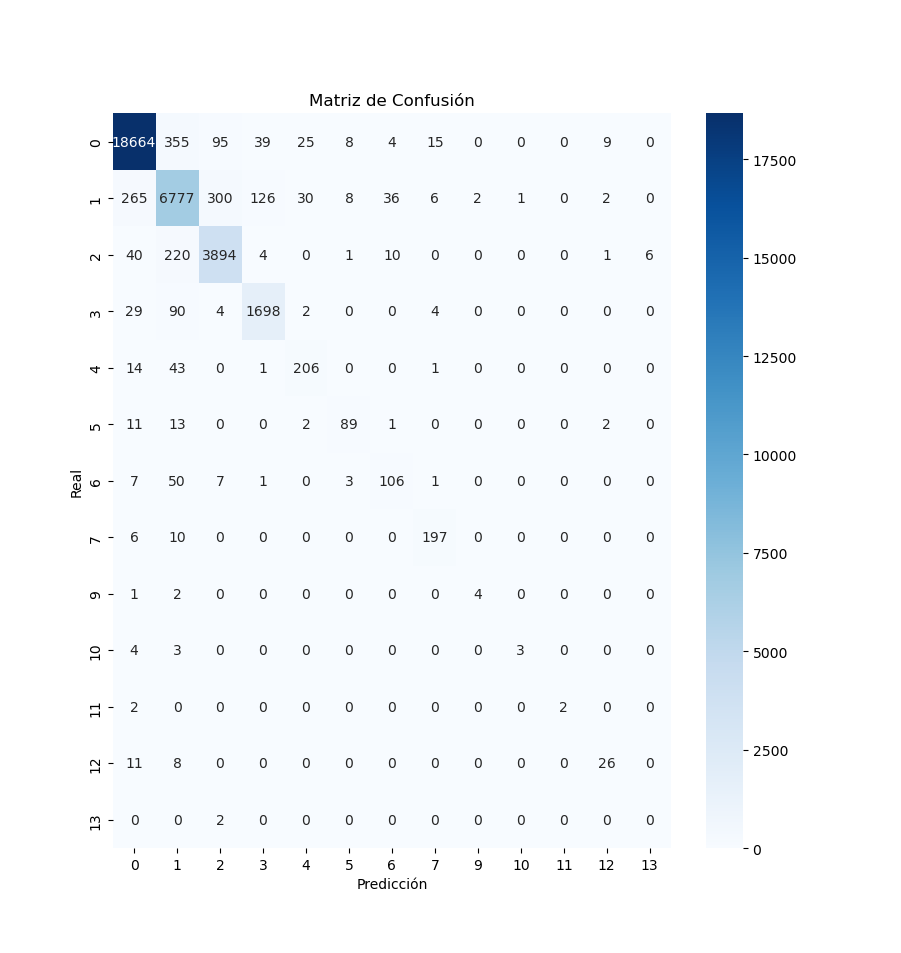
\includegraphics[width=1.2\linewidth]{Imagenes/confusion_multiclase}
	\caption[Matriz de confusión para la clasificación multicase]{Matriz de confusión para la clasificación multicase}
	\label{fig:confusion}
\end{figure}

Según el estudio \textit{Malware Behavior Analysis: Learning and Understanding Current Malware Threats} \cite{mba}, algunos de los tipos de \textit{malware} que tenemos con menos patrones, se pueden agrupar en algunas de las clases más representadas de nuestro conjunto de datos. En este estudio se comenta que \textit{p2p-worm} añade un comportamiento específico al comportamiento de un gusano, generando problemas de red y de pérdida de datos. Algo similar pasa con \textit{Gamethief trojan}. De esta forma podemos agrupar estos patrones a sus respectivas clases similares sin perder efectividad a la hora de clasificar y además eliminar así dos de las clases que nos pueden dar problemas por falta de información.

\vspace{1em}

Por otro lado, se han planteado dos formas de solucionar este problema, aunque ambas presentan inconvenientes:

\begin{itemize}
	\item Eliminar las clases menos representadas. Tiene el riesgo de no reconocer un nuevo patrón si es de un tipo distinto de \textit{malware}.
	\item Agruparlas en una nueva clase que represente varios tipos de \textit{malware}. En este caso estamos suponiendo que los patrones agrupados tienen unas características similares.
\end{itemize}

\vspace{1em}

Finalmente hemos decidido agrupar las clases con menos de 30 patrones en una nueva categoría \textit{otros}. Por número de patrones sería recomendable agrupar también la clase \textit{virus}, pero podría tener demasiado peso en la categoría otros y hemos considerado que es lo suficientemente relevante como para estudiarla por separado. En la tabla \ref{tabla:multi_new} podemos ver que, aunque mejoramos la mínima sensibilidad, no se producen unas mejoras significativas en la precisión de clasificación pero dada la alta precisión presentada por los modelos y la mejora en la mínima sensibilidad puede considerarse una buena actualización. Podemos ver la nueva codificación en la tabla \ref{tabla:nueva_codificacion_malware}

\begin{table}[th]
	\centering
	\begin{tabular}{ |m{4cm}|c|c| }
		\hline
		\rowcolor{LightCyan}
		Categoría                   & Codificación & Nº de patrones \\
		\hline
		\textit{benign}             & 0            & 77142 \\
		\textit{trojan}             & 1            & 29978 \\
		\textit{worm}               & 2            & 16713 \\
		\textit{backdoor}           & 3            & 7331  \\
		\textit{downloader}         & 4            & 1031  \\
		\textit{informationstealer} & 5            & 448   \\
		\textit{dropper}            & 6            & 715   \\
		\textit{ransomware}         & 7            & 821   \\
		\textit{virus}              & 8            & 192   \\
		\textit{otros}              & 9            & 64    \\
		\hline
	\end{tabular}
	\caption{Nueva codificación de las clases \textit{malware}.}
	\label{tabla:nueva_codificacion_malware}
\end{table}

\begin{table}[th]
	\centering
	\begin{tabular}{ |c|c|c|c|c|c|c|c| }
		\hline
		\rowcolor{LightCyan}
		Clasificador & Tiempo (s) & \multicolumn{3}{c|}{Entrenamiento} & \multicolumn{3}{c|}{Test} \\
		\hline
		\rowcolor{LightCyan}
		&            & Acc & MS & F1 & Acc & MS & F1 \\
		\hline
		\textit{Decission tree} & 1.220  & 0.998 & 0.992 & 0.998 & 0.938 & 0.670 & 0.975 \\
		\textit{Random forest}  & 31.201 & 0.998 & 0.993 & 0.998 & 0.953 & 0.670 & 0.980 \\
		\textit{K-NN}           & 0.083  & 0.951 & 0.431 & 0.980 & 0.936 & 0.333 & 0.974 \\
		\hline
	\end{tabular}
	\caption{Clasificación multiclase con la nueva codificación.}
	\label{tabla:multi_new}
\end{table}

\vspace{1em}

Por último, se han considerado otras opciones para mejorar la clasificación de las clases minoritarias, pero podrían exceder la complejidad de este proyecto:

\begin{itemize}
	\item Utilizar métodos de sobremuestreo, ya mencionados en la sección \ref{subsubsec:oversampling}, que consisten en aumentar la cantidad de patrones de estas clases de forma sintética.
	\item Utilizar métodos jerárquicos que primero clasifiquen usando la categoría \textit{otros}, para después dividirla en sus diferentes clases y entrenar un modelo específico.
\end{itemize}

\section{Preparación del entorno}
\label{sec:prep_entorno}

En esta sección se describe el entorno de trabajo utilizado por el alumno para la implementación de los modelos y la realización de las pruebas. El entorno se debe preparar de forma correcta, ya que puede afectar a la ejecución de los algoritmos y a la reproducibilidad de los experimentos. A continuación, se explican elementos del entorno como el lenguaje de programación, las bibliotecas y las características del equipo.

\subsection{Herramientas y bibliotecas}
\label{subsec:herramientas}

El desarrollo y la experimentación de este proyecto se han llevado a cabo empleando un conjunto de herramientas y bibliotecas muy utilizadas en la ciencia de datos. \textit{Python} ha sido el lenguaje de programación de este trabajo, ya que ofrece una fácil implementación de modelos, manipulación de datos y visualización de resultados. Su popularidad en se debe a su sintaxis sencilla, escalabilidad y amplia variedad de herramientas y bibliotecas \cite{python_ml}.

\vspace{1em}

En este proyecto se ha utilizado la versión 3.12 de \textit{Python}, elegida principalmente por su compatibilidad con las bibliotecas empleadas, en particular, con \textit{GridSearchCV}, que aprovechan la paralelización de procesos para mejorar el rendimiento. El problema encontrado es que los hilos no se cierran correctamente, es un comportamiento típico asociado a lo que en programación concurrente se denomina \textit{thread leakage} o hilos huérfanos. provoca que la memoria \textit{RAM} y la \textit{CPU} sigan siendo consumidas incluso después de que la ejecución haya terminado. En teoría, este problema no afecta al rendimiento de los clasificadores, pero puede afectar al tiempo de ejecución.

\vspace{1em}

Las bibliotecas utilizadas para construir un modelo y analizar los datos son \textit{Scikit-learn}, \textit{DLOrdinal}, \textit{Matplotlib}, \textit{NumPy}, \textit{Pandas}, \textit{LightGBM} y \textit{Seaborn}.

\subsubsection{\textit{Scikit-learn}}
\label{subsubsec:sklearn}

\textit{Scikit-learn} es un paquete de código abierto en \textit{Python} que ofrece una gran variedad de métodos de aprendizaje automático rápidos y eficientes, gracias a que usan bibliotecas compiladas en lenguajes como \textit{C++}, \textit{C} o \textit{Fortran}. Tiene detrás una comunidad activa que mantiene la documentación, corrige errores y asegura la calidad. Aunque no incluye todos los algoritmos usados en este proyecto, es una herramienta muy recomendable si necesitamos: transformación de datos, aprendizaje supervisado o evaluación de modelos \cite{hao2019scikit}.

\subsubsection{\textit{DLOrdinal}}
\label{subsubsec:dlordinal}

La biblioteca dlordinal incluye muchas de las metodologías más recientes de clasificación ordinal usando técnicas avanzadas de aprendizaje profundo. El enfoque ordinal de esta herramienta tiene el objetivo de aprovechar la información de orden presente en la variable objetivo usando funciones de pérdida, diversas capas de salida y otras estrategias \cite{dlordinal}. El módulo de dlordinal que nos ha resultado de utilidad para este proyecto ha sido la el conjunto de métricas que incluye para evaluar los modelos utilizados, ya que cuenta con algunas de las métricas que finalmente hemos usado: mínima sensibilidad y valor-F.

\subsubsection{\textit{Matplotlib}}
\label{subsubsec:matplotlib}

Para una mejor visualización de los datos obtenidos en los modelos utilizados, se ha usado la biblioteca Matplotlib, ya que incluye una gran cantidad de recursos para la representación gráfica de la información \cite{matplotlib}. Se ha usado, en combinación con \textit{Seaborn}, descrita en la sección \ref{subsubsec:seaborn}.

\subsubsection{\textit{NumPy}}
\label{subsubsec:numpy}

La biblioteca \textit{NumPy} tiene como objetivo principal dar soporte a la creación de vectores y matrices de grandes dimensiones, junto con una colección de funciones matemáticas con las que operar \cite{numpy}. Ha sido de gran utilidad en el desarrollo del proyecto, ya que el conjunto de datos con el que se ha trabajado es de un tamaño considerable, aunque no ha sido necesario hacer uso de las funciones que proporciona porque la mayor parte de los cálculos necesarios se hacen de manera interna en los modelos utilizados.

\subsubsection{\textit{Pandas}}
\label{subsubsec:pandas}

Pandas es una herramienta muy potente para el manejo, análisis y manipulación de datos. Incluye una amplia variedad de herramientas para: leer y escribir datos, reestructuración y segmentación, inserción y eliminación de columnas, mezcla y unión de datos y muchas funcionalidades más \cite{pandas}. Varias de ellas se han utilizado durante el desarrollo y la preparación del conjunto de datos.

\subsubsection{\textit{LightGBM}}
\label{subsubsec:lightgbm}

La biblioteca \textit{Light Gradient-Boosting Machine} por su nombre en inglés, es una infraestructura de aprendizaje automático basada en modelos de árboles de decisión \cite{lgbm}. Se puede usar en diferentes tareas, pero la importante para el análisis realizado el la de clasificación. Los principales algoritmos soportados son: \textit{Gradient Boosting Decision Trees (GBDT)}, el cual utiliza \textit{LGBMClassifier}, clasificador usado durante la experimentación, \textit{Dropouts meet Multiple Additive Regression Trees (Dart)} y \textit{Gradient-based One-Side Sampling (Goss)} \cite{lgbm_alg}.

\subsubsection{\textit{Seaborn}}
\label{subsubsec:seaborn}

Basada en \textit{Matplotlib}, \textit{Seaborn} proporciona una interfaz de alto nivel para generar gráficos estadisticos \cite{seaborn}. Es posible usar ambas bibliotecas de forma combinada para una mayor capacidad de visualización. Mientras que \textit{Matplotlib} ofrece un control detallado sobre cada elemento de la figura, \textit{Seaborn} simplifica la creación de visualizaciones complejas, incorporando estilos predefinidos y funciones específicas para el análisis de datos.

\subsection{Hardware}
\label{subsec:hw_usado}

El entrenamiento y evaluación de los modelos se ha realizado en el equipo del estudiante con las siguientes características: procesador \textit{Intel Core i7-4712MQ}, tarjeta gráfica \textit{NVIDIA GeForce 920M}, 16 GB de \textit{RAM} DDR3 y almacenamiento compuesto por un \textit{SSD Crucial MX500} de 250 GB y un \textit{HDD} de 1 TB. Este hardware permite la paralelización de los algoritmos en múltiples núcleos del procesador, lo que reduce significativamente los tiempos de entrenamiento, pero se encuentra muy limitado respecto al conjunto utilizado para clasificación multiclase y modelos más costosos como puede ser \textit{SVM}.

\subsection{Protocolo de experimentación y validación}
\label{subsec:protocolo_exper}

En esta sección se establecen las condiciones de evaluación del rendimiento de los modelos mencionados en la sección \ref{sec:modelos_utilizados} y se explican los procedimientos seguidos, las técnicas de validación usadas y los criterios que permiten medir de forma objetiva la calidad de las predicciones. Todo esto tiene objetivo de minimizar posibles sesgos, evitar el sobreajuste y obtener conclusiones fiables.

\subsubsection{Diseño experimental}
\label{subsubsec:diseño}

Inicialmente se han planteado tres formas de estructurar el diseño experimental y como se evaluarán posteriormente las pruebas. La primera ha sido comparar distintos modelos para cada tipo de clasificación. La segunda, comparar, clasificación binaria y multiclase para cada clasificador. Por último, se ha planteado la posibilidad de una combinación de ambas comparaciones. Este último caso se ha descarta porque, aunque puede ser interesante la comparación combinada por proporcionar una amplia visión del problema, duplica la carga de trabajo y puede exceder la complejidad del proyecto.

\vspace{1em}

La segunda opción planteada puede servir para comparar el rendimiento de uno o varios modelos según la naturaleza del problema y realizar un análisis de coste computacional. Son aspectos interesantes a estudiar, pero no entran dentro de los objetivos de este estudio.

\vspace{1em}

Finalmente se ha seleccionado la primera opción. Aunque el problema de la detección de malware puede enfocarse tanto para la simple detección de un programa malicioso como para identificar a que tipo pertenece, los problemas de clasificación binaria y multiclase tienen enfoques muy diferentes. Por otro lado, el conjunto de datos usado para clasificación multiclase contiene varias clases con muy pocos patrones y la comparación podría no ser justa.

\subsubsection{Validación de resultados}
\label{subsubsec:validacion}

Para evitar sesgos y resultados poco concluyentes se han empleado varias técnicas.

\begin{itemize}
	\item \textbf{Validación cruzada}: Se ha usado el parámetro \textit{cv} de \textit{GridSearchCV}. En general se han usado 5, aunque en algunos casos ha sido necesario ajustarlo por tiempo.
	\item \textbf{Validación cruzada estratificada adaptativa}: la función \textit{cv()} que encontramos en el Anexo \ref{sec:func_cv} ajusta el numero de particiones en caso de que una clase tenga menos muestras que particiones indicadas.
	\item \textbf{Particion entrenamiento/prueba}: se ha dividido el conjunto de datos en un 75-25 para entrenamiento y pruebas respectivamente usando la variable \textit{random\_state} con la semilla usada en las pruebas.
	\item \textbf{Repetición con semillas aleatorias}: para repetir los experimentos y tener una visión más amplia.
	\item \textbf{Ajuste de pesos de clase}: mediante \texttt{class\_weight = "balanced"} en los clasificadores en los que se encuentra disponible.
\end{itemize}

A pesar de todas estas técnicas, es bastante probable que las clases extremadamente minoritarias del conjunto de datos para la clasificación multiclase pueden tener una influencia muy limitada.

\subsubsection{Reproducibilidad}
\label{subsubsec:reproducibilidad}

Durante el desarrollo del código y de las pruebas, se han adoptado diferentes medidas para garantizar que las comparaciones entre modelos sean justas.

\begin{enumerate}
	\item \textbf{Fijación de semillas:}\\
		Se ha hecho uso de una semilla controlada dentro de un bucle para repetir el experimento. Con ella se controla:

		\begin{itemize}
			\item La partición aleatoria de test y entrenamiento.
			\item la inicialización interna de los clasificadores que aceptan \textit{randon\_state}.
		\end{itemize}
	\item \textbf{Número de repeticiones:}\\
		Si bien el número de repeticiones es ajustable dentro del código utilizado, para asegurar una justa comparación y por las limitaciones del equipo, se han usado 10 semillas en todos los experimentos. Esto permite obtener la media y la desviación típica de las métricas y reducir la variabilidad.
	\item \textbf{Control de parámetros:}\\
		Los hiperparámetros se optimizan con \textit{GridSearchCV} usando la misma rejilla para todas las semillas para poder tener una comparación coherente.
\end{enumerate}

Estas medidas permiten obtener los mismo resultados si se usan las mismas semillas, configuraciones y conjunto de datos.

\subsubsection{Control de parámetros}
\label{subsubsec:control}

Para la optimización de hiperparámetros hemos usado búsqueda en rejilla de \textit{GridSearchCV}. Esta técnica hace pruebas con todas las combinaciones posibles de los parámetros proporcionados y usa validación cruzada para garantizar la robustez de los resultados. El problema con esta técnica es el elevado número de pruebas, ya que se prueban todas las combinaciones de parámetros posibles en cada uno de los conjuntos de la validación cruzada, lo que eleva el tiempo necesario de manera considerable.

\vspace{1em}

Una opción considerada y probada para evitar esta limitación es la búsqueda aleatoria de \textit{RandomizedSearchCV}, que permite establecer un número máximo de combinaciones a probar y puede reducir considerablemente el número de combinaciones evaluadas. El inconveniente que ha surgido con esta técnica es que al disponer de un \textit{Hardware} muy limitado, la cantidad de combinaciones usadas es pequeña y limitar aun más con la búsqueda aleatoria puede suponer que los resultados sean menos representativos.

\vspace{1em}

La rejilla se ha establecido para cada modelo en función de las limitaciones del equipo, el tiempo necesario para el entrenamiento de cada modelo y cuanto influye ese parámetro en el tiempo de entrenamiento y el peso que tiene en los resultados.

\subsubsection{Criterios de evaluación}
\label{subsubsec:evaluacion}

Para evaluar la efectividad de los modelos implementados, se han utilizado las siguientes métricas, cuya descripción teórica se encuentra en la sección \ref{subsec:2_metricas}:

\begin{itemize}
	\item \textbf{\textit{Accuracy}}: proporción de predicciones correctas sobre el total de patrones.
	\item \textbf{Mínima Sensibilidad}: sensibilidad de la clase peor clasificada.
	\item \textbf{\textit{F1-score}}: media armónica entre precisión y sensibilidad. En este documento se ha hecho referencia a ella como valor-F.
\end{itemize}

\section{Implementación y pruebas}
\label{sec:implementacion}

En esta sección se describe, principalmente, la estructura del código empleado para realizar los experimentos y el procedimiento seguido dentro del mismo para entrenar y evaluar los modelos seleccionados. Además se va a tratar la preparación del conjunto de datos, es decir, cómo se cargan y cómo se divide la información para realizar el entrenamiento y las pruebas. Por último, se tratará la forma que hemos seguido para presentar los resultados y las métricas que se han mencionado en la sección \ref{subsubsec:evaluacion}

\subsection{Estructura del código}
\label{subsec:estructura_codigo}
% TODO: Se describe cómo se organizan los scripts y módulos, indicando la función de cada uno en el flujo de entrenamiento, evaluación y análisis de resultados.



\subsection{Procedimiento de entrenamiento y evaluación}
\label{subsec:procedimiento}

El planteamiento seguido para entrenar los diferentes modelos ha sido usar \textit{GridSearchCV} para ajustar los modelos de clasificación con los mejores parámetros posibles. Para obtener una visión más amplia y más justa del problema, se ha repetido el entrenamiento, con las mismas 10 semillas para todos los modelos. Con esto conseguimos que el experimento sea controlado y reproducible, ya que para un mismo modelo, una misma semilla y la misma rejilla de parámetros, obtendremos siempre los mismos resultados. Una vez calculadas las métricas seleccionadas en la sección \ref{subsubsec:evaluacion}, se calcula la media y la desviación típica de todas ellas para usarlas como valor final de comparación entre modelos.

\subsection{Preparación y uso de los conjuntos de datos}
\label{subsec:datos_experimentales}

Además del tratamiento previo del conjunto de datos realizado en la sección \ref{sec:proc_dataset}, es necesario procesar la información antes de entrenar. Con la función \textit{load}, cargamos el conjunto de datos en dos matrices de \textit{Numpy}, la matriz de información y la matriz de clases. La matriz de patrones de entrada se normaliza haciendo uso de la clase \textit{MinMaxScaler} del módulo \textit{preprocessing} de \textit{Scikit-Learn}. Por último, haciendo uso de la función \textit{train\_test\_split}, dividimos el conjunto de datos en test y entrenamiento. Esto se hace dentro del bucle y para cada semilla con el objetivo de tener una evaluación más robusta, ya que permite tener una división distinta y controlada para cada semilla.

\subsection{Métricas y análisis de resultados}
\label{subsec:metricas_pruebas}

Para calcular las métricas se han usado las funciones \textit{accuracy\_off1} y \textit{minimum\_sensitivity} para las métricas valor-F y mínima sensibilidad respectivamente. Estas se encuentran disponibles en el módulo \textit{metrics} de la librería \textit{dlordinal}. Para calcular la exactitud o \textit{accuracy} del entrenamiento, se ha usado la función \textit{accuracy\_score} disponible en el módulo \textit{metrics} de la librería \textit{Scikit-Learn}. Finalmente, una vez calculados los resultados para todas las semillas, se guardan en un objeto \textit{DataFrame} de \textit{Pandas} con el formato que se muestra en el ejemplo del Anexo \ref{sec:info}. Haciendo uso de los métodos \textit{mean} y \textit{std} de esta clase, se obtiene la media y la desviación típica de todas las semillas.

\chapter{Resultados y discusión}
\label{ch:resultados}
\chapter{Conclusiones y recomendaciones}
\label{ch:conclusiones}

% --> poner otros capítulos. Por ejemplo:
	%\input{2_objetivos}
	%\input{3_antecedentes}
	%\input{4_materiales}
	%\input{5_diseno}
	%\input{6_pruebas}
	%\chapter{Ejemplos de código Latex}
\label{ch:codigos_ejemplo}
Aquí también se puede poner texto.

\section{Acrónimos}
Ejemplo de como poner un acrónimo \acrshort{iot}. Estos están definidos en el archivo ``anexo\_acronimos.text''.


\section{Comillas}
Mira el código para que veas como se hace bien el ``entrecomillado''. No se usan las comillas situadas en la tecla del dígito 2.

\section{Listas}
En esta sección se muestra como crear dos tipos de listas.

\subsection{Lista Enumerada}
\begin{enumerate}
\item Color rojo
\item Color verde
\item Color amarillo
\end{enumerate}



\subsection{Lista NO-Enumerada}
\begin{itemize}
\item Color rojo
\item Color verde
\item Color amarillo
\end{itemize}

\section{Como incluir FIGURAS}

\subsection{Figura única}
\label{sec:figura_unica}

\begin{figure}[H]
  \centering
  % include first image
  
\includegraphics[width=.8\linewidth]{Imagenes/logo_uco}  
  \caption[Titulo de la figura para el índice de figuras. En este no se deben poner referencias a citas]{Título de la figura para el texto}
  \label{fig:figura_unica}
\end{figure}

\subsection{Figura con subfiguras}

En la Figura \ref{figT:subfiguras} se puede aprecia una figura compuesta por dos subfiguras.

\begin{figure}[H]
\begin{subfigure}{.5\textwidth}
  \centering
  % include first image
  
\includegraphics[width=.8\linewidth]{Imagenes/logo_uco}  
  \caption{Título subfigura 1}
  \label{fig:sub-first}
\end{subfigure}
\begin{subfigure}{.5\textwidth}
  \centering
  % include second image
  
\includegraphics[width=.8\linewidth]{Imagenes/logo_uco}  
  \caption{Título subfigura 2}
  \label{fig:sub-second}
\end{subfigure}
\caption{Titulo principal figura}
\label{figT:subfiguras}
\end{figure}

\subsection{Figura con subfiguras en distintas líneas}
\begin{figure}[H]
\begin{subfigure}{.5\textwidth}
  \centering
  % include first image
  
\includegraphics[width=.8\linewidth]{Imagenes/logo_uco}  
  \caption{Título subfigura 1}
  \label{fig:sub-first}
\end{subfigure}
\begin{subfigure}{.5\textwidth}
  \centering
  % include second image
  
\includegraphics[width=.8\linewidth]{Imagenes/logo_uco}  
  \caption{Título subfigura 2}
  \label{fig:sub-second}
\end{subfigure}

\begin{subfigure}{.5\textwidth}
  \centering
  % include first image
  
\includegraphics[width=.8\linewidth]{Imagenes/logo_uco}  
  \caption{Título subfigura 3}
  \label{fig:sub-first}
\end{subfigure}
\begin{subfigure}{.5\textwidth}
  \centering
  % include second image
  
\includegraphics[width=.8\linewidth]{Imagenes/logo_uco}  
  \caption{Título subfigura 4}
  \label{fig:sub-second}
\end{subfigure}

\caption{Figuras en multiples lineas}
\label{figT:subfiguras2}
\end{figure}


\section{Fórmulas Matemáticas}

\subsection{Formulas referenciables}
\begin{equation} \label{eq:erl} a = bq + r \end{equation} donde \eqref{eq:erl} es verdadera si $a$ y $b$ son enteros con $b \neq c$. 

\subsection{Fórmulas que no se van a referenciar}
\begin{align*} 
X = 0,42 \ \tau_{625} + 0.35 \ \tau_{550} + 0.21 \ \tau_{445} \\
Y = 0,20 \ \tau_{625} + 0.63 \ \tau_{550} + 0.17 \ \tau_{495} \\
Z = 0,24 \ \tau_{495} + 0.94 \ \tau_{445} 
\end{align*}

Y con estos valores se calculan las coordenadas \textit{x} e \textit{y}:

\begin{align*} 
x = X / (X + Y + Z) \quad y = Y / (X + Y + Z)
\end{align*}

\section{Diagramas usando TikZ}
\url{https://es.overleaf.com/learn/latex/LaTeX_Graphics_using_TikZ%3A_A_Tutorial_for_Beginners_(Part_1)%E2%80%94Basic_Drawing}

\subsection{Ejemplo diagrama de flujo}

\begin{diagrama}
\centering
 
    \begin{tikzpicture}[node distance=2cm]

    \node (start) [startstop] {Start};
    \node (in1) [io, below of=start] {Input};
    \node (pro1) [process, below of=in1] {Process 1};
    \node (dec1) [decision, below of=pro1, yshift=-0.5cm] {Decision 1};

    \node (pro2a) [process, below of=dec1, yshift=-0.5cm] {Process 2a text text text text text text text};

    \node (pro2b) [process, right of=dec1, xshift=2cm] {Process 2b};
    \node (out1) [io, below of=pro2a] {Output};
    \node (stop) [startstop, below of=out1] {Stop};

    \draw [arrow] (start) -- (in1);
    \draw [arrow] (in1) -- (pro1);
    \draw [arrow] (pro1) -- (dec1);
    \draw [arrow] (dec1) -- node[anchor=east] {yes} (pro2a);
    \draw [arrow] (dec1) -- node[anchor=south] {no} (pro2b);
    \draw [arrow] (pro2b) |- (pro1);
    \draw [arrow] (pro2a) -- (out1);
    \draw [arrow] (out1) -- (stop);

    \end{tikzpicture}

	\caption{Ejemplo diagrama}
	\label{diagrama:ejemplo_diagrama}
\end{diagrama}

\section{Referencia a distintas secciones y figuras}
En la sección \ref{sec:figura_unica} se puede ver la Figura \ref{fig:figura_unica}.

En el capítulo \ref{ch:presupuesto} se puede ver el código para crear una tabla. La Tabla \ref{tabla:presupuesto} muestra un presupuesto.
	%\chapter{Resultados y discusión}
\label{ch:resultados}



%--------------------%
% DOCUMENTOS TÉNICOS %
%--------------------%

%\chapter*{PRESUPUESTO}
\label{ch:presupuesto}

\addcontentsline{toc}{chapter}{Presupuesto} % si queremos que aparezca en el índice
\markboth{PRESUPUESTO}{PRESUPUESTO} % encabezado

En esta seccion, se presentan los gastos asociados al desarrollo del presente proyecto, los cuales se refieren exclusivamente a los elementos que conforman la parte hardware del sistema.

%\clearpage

\definecolor{LightCyan}{rgb}{0.88,1,1}

\begin{table}[ht]
	\centering
	\begin{tabular}{ |m{7cm}|c|r|r| }
		\hline
		\rowcolor{LightCyan}
		Descripción & Cantidad & Precio (\euro) & Importe (\euro)\\
		\hline
		Pantalla LCD Quimat 20x4 & 1 & 10,69 & 10,69\\
		\hline
		Baterías 9 V & 3 & 2,10 & 6,36\\
		\hline
		Amplificador operacional TL082IP & 3 & 0,61 & 1,84\\
		\hline
		Regulador tensión L7905CV  & 1 & 0,40 &  0,40\\
		\hline
		Resistencias $20 M\Omega$ & 1 & 0,60 & 0,60\\
		\hline
		Resistencias $5M \Omega$ & 1 & 0,85 & 0,85\\
		\hline
		Condensadores $2.2 \mu F$ & 1 & 0,37 & 0,37 \\
		\hline
		Condensadores $1 \mu F$ & 1 & 0,20 & 0,20\\
		\hline
		Condensadores $1 \rho F$ & 3 & 0,35 & 1,05\\
		\hline
		Transistor BJT 2N3904 & 6 & 0,40 & 2,4 \\
		\hline
		Placas de prototipado & 2 & 3,00 & 6,00\\
		\hline
		\textbf{Total} &  &  & \textbf{59,90 \euro}\\
		\hline
	\end{tabular}
	\caption{Presupuesto del proyecto.}
	\label{tabla:presupuesto}
\end{table}




%------------------%
%	BIBLIOGRAFIA   %
%------------------%

%Estilo de la bibliografia
\bibliographystyle{unsrtnat}
%\bibliographystyle{elsarticle-num}
\bibliography{referencias.bib}

%------------------%
%      ANEXOS      %
%------------------%

%\chapter*{PLANOS}

\addcontentsline{toc}{chapter}{Planos} % si queremos que aparezca en el índice
\markboth{PLANOS}{PLANOS} % encabezado


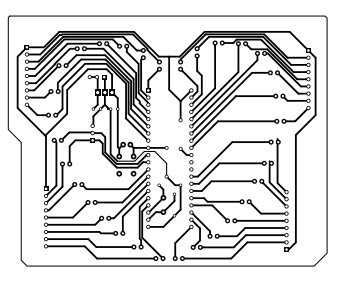
\includepdf[scale=0.8,pages=1,angle=90,pagecommand=\section*{Placa de Circuito Impreso (PCB)}\label{planos:PCB}]{DocumentacionTecnica/ejemplo_pcb.png}


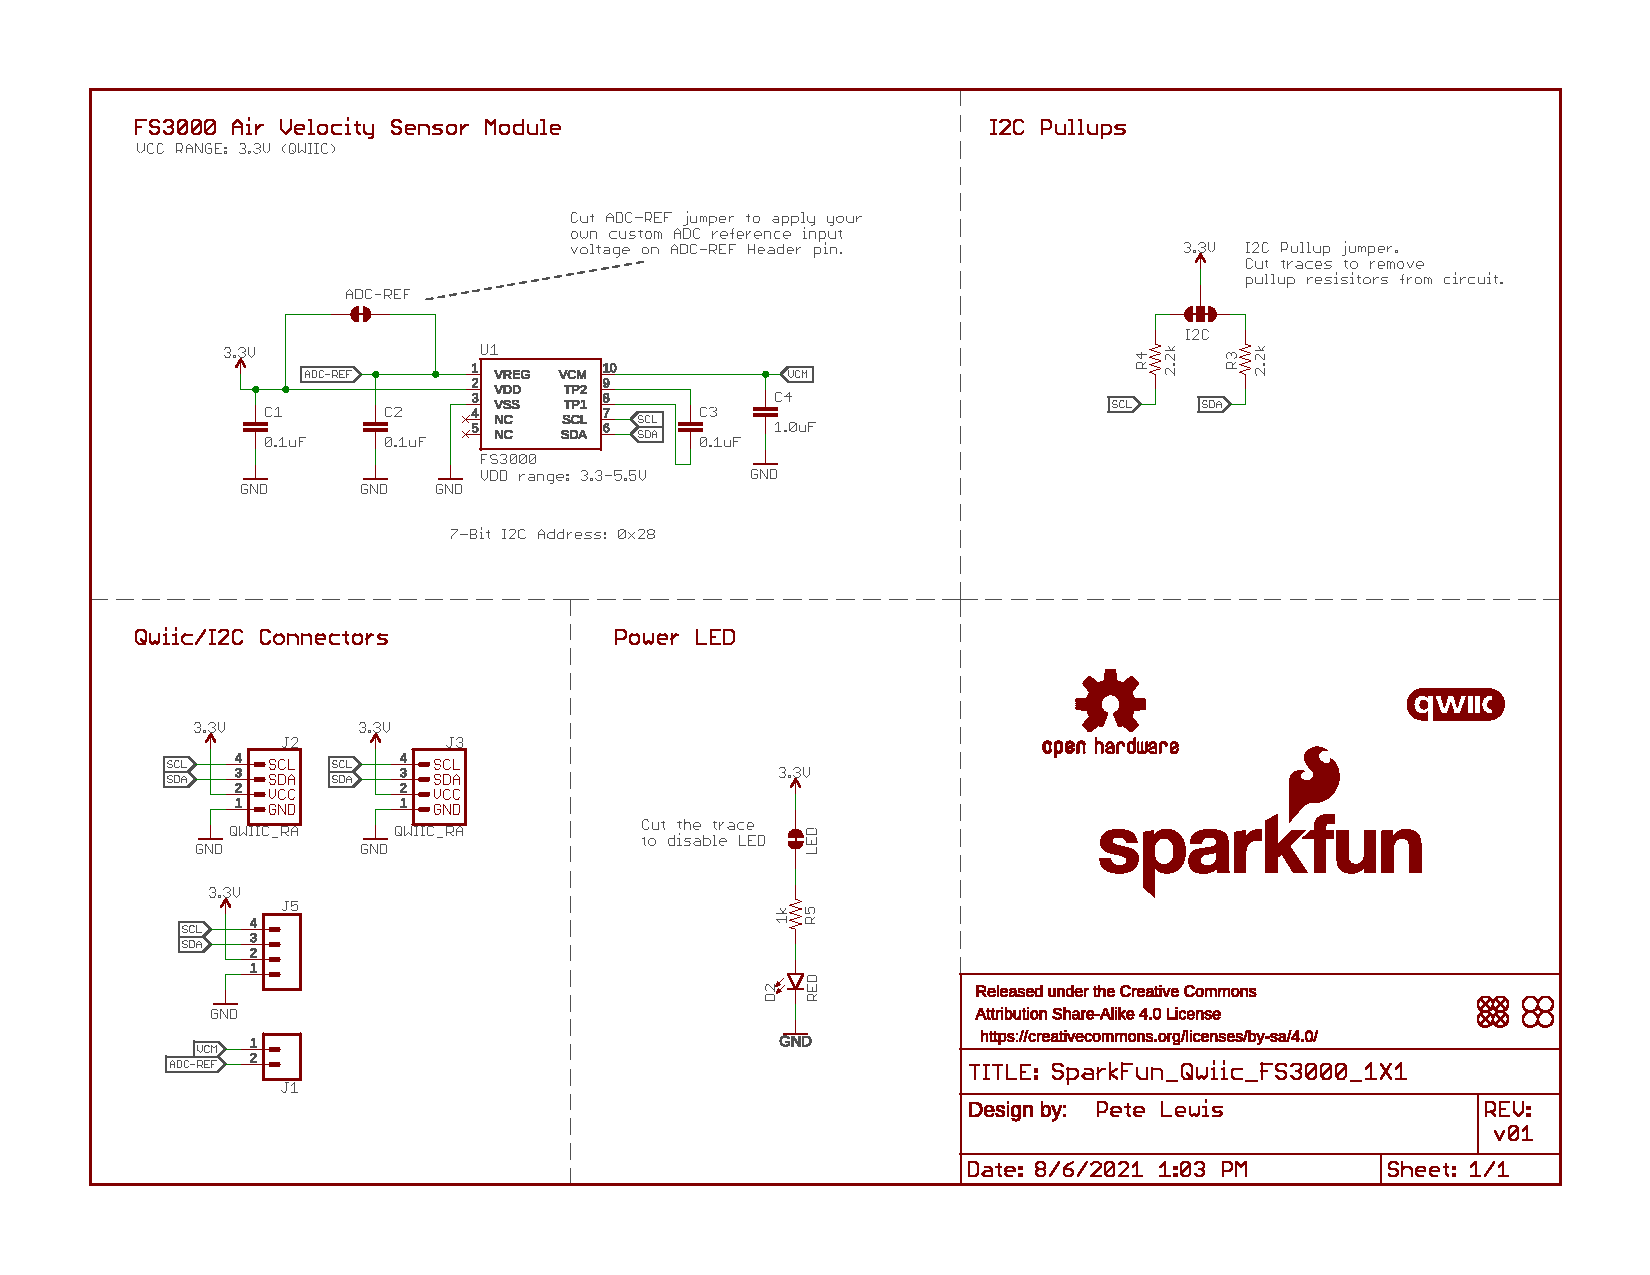
\includepdf[scale=0.8,pages=1,angle=90,pagecommand=\section*{Esquema Eléctrico}\label{planos:esquema_electrico}]{DocumentacionTecnica/Ejemplo_Esquema_Electrico.pdf}

\appendix

% \chapter{Hojas de Características}

% Pages: Es este parámetro se indican cuantas páginas se quieren poner 1 o 1-2, ...
% Angle: A veces es necesario rotar la página --> angle=90
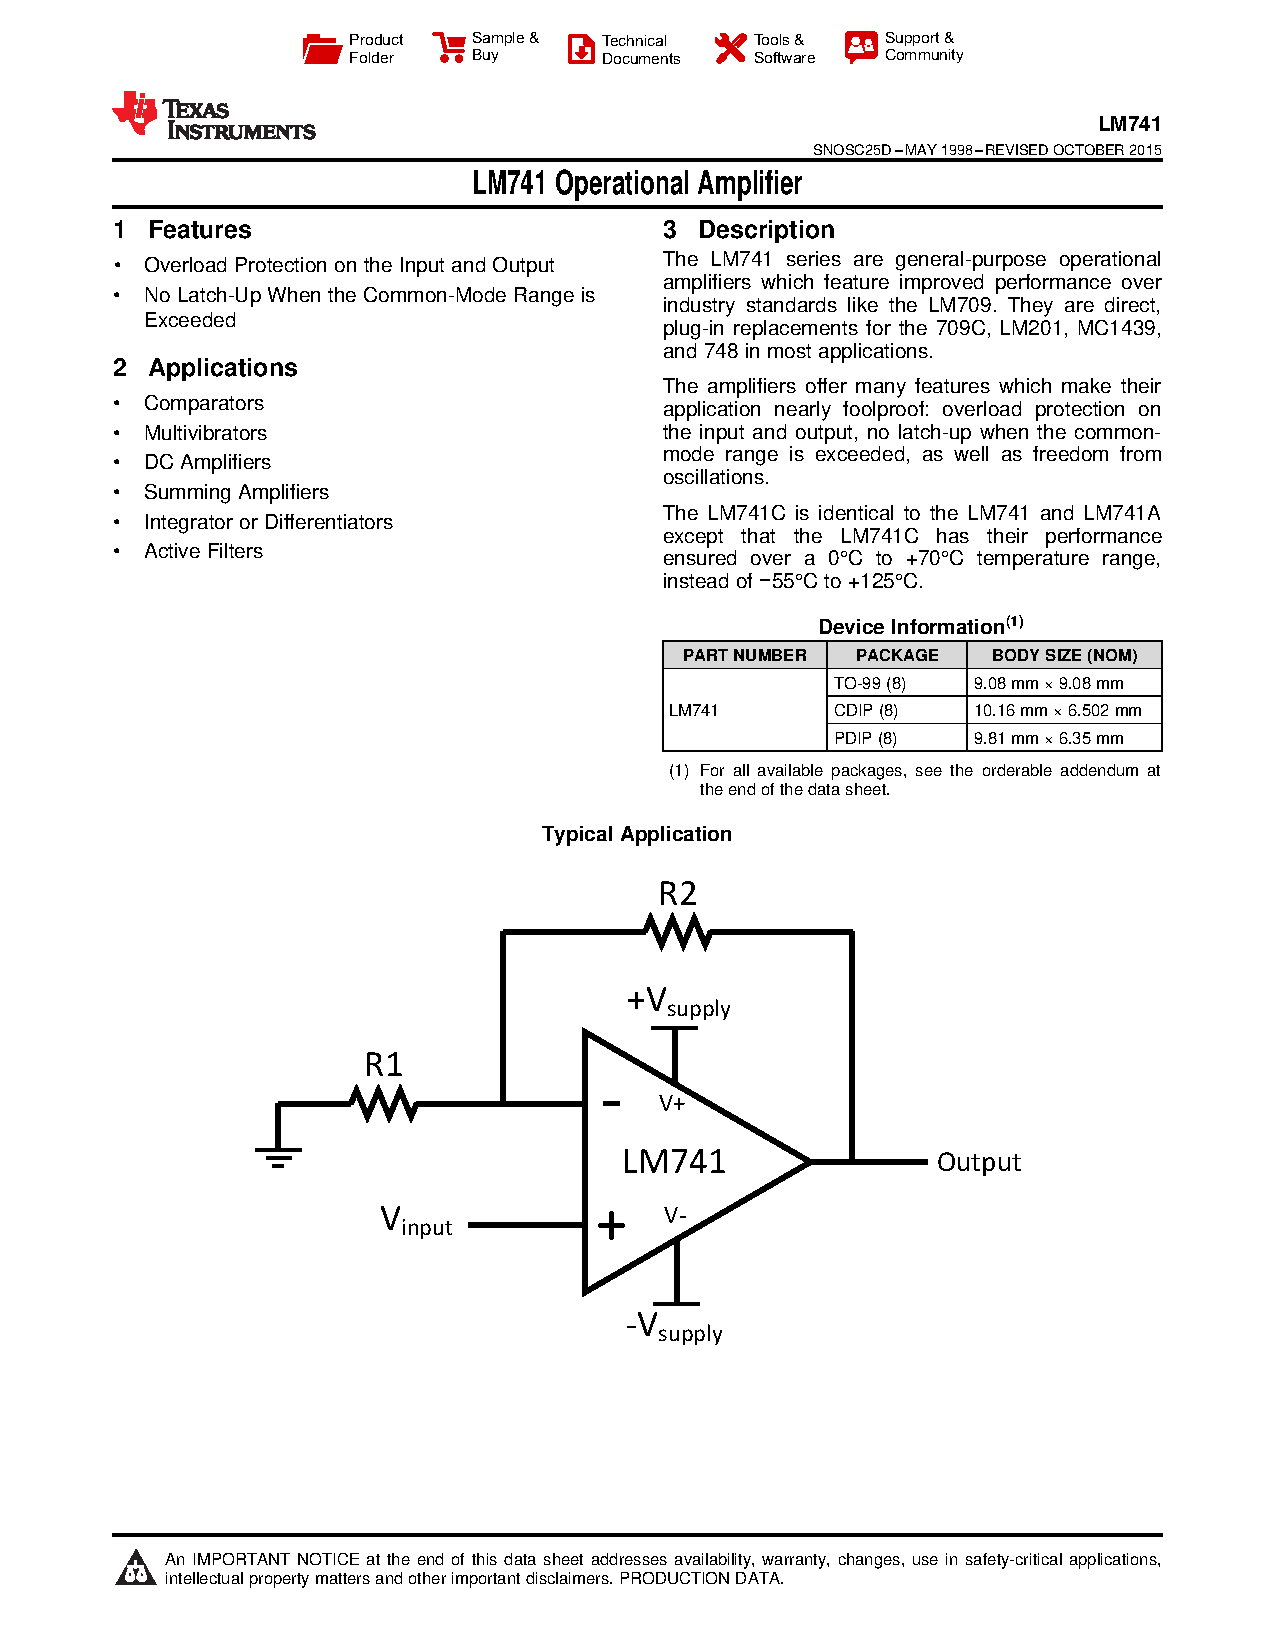
\includepdf[scale=0.7,pages=1,angle=0,pagecommand=\section{Amplificador Operacional 741}\label{hc:ao_741}]{HojasDeCaracteristicas/ejemplo_lm741.pdf}
\chapter{Código del programa}


\section{Codificación de las categorías \textit{malware}}
\label{sec:codificacion}

\lstset{style=codestyle, language=Python}
\begin{lstlisting}[frame=single]
X, y        = load('bodmas/bodmas.npz')
metadata    = pd.read_csv('bodmas/bodmas_metadata.csv')
mw_category = pd.read_csv('bodmas/bodmas_malware_category.csv')

# Incluimos los valores de 'category' en metadata cuando coinciden los valoes de 'sha'
mw_category = metadata.merge(mw_category, on = 'sha', how = 'left')

# Rellenamos los huecos como software benigno
mw_category['category'] = mw_category['category'].fillna('benign')

# Eliminamos todas las columnas excepto 'category'
mw_category = mw_category['category']

# Codificamos las categorias de malware
category = {
	'benign': 0, 'trojan': 1, 'worm': 2, 'backdoor': 3,
	'downloader': 4, 'informationstealer': 5, 'dropper': 6,
	'ransomware': 7, 'rootkit': 8, 'cryptominer': 9, 'pua': 10,
	'exploit': 11, 'virus': 12, 'p2p-worm': 13, 'trojan-gamethief': 14
}

mw_category = mw_category.map(category)

y = mw_category.to_numpy()

save('bodmas/bodmas_multiclass.npz', X, y)

\end{lstlisting}

\section{Reducción de la dimensionalidad}
\label{sec:red_dim}

\lstset{style=codestyle, language=Python}
\begin{lstlisting}[frame=single]
def resampling(X, y, n_components = 5, size = 15000, u = False):
	if u:
		rus  = RandomUnderSampler(sampling_strategy = {0: size, 1: size})
		# rus  = RandomUnderSampler(sampling_strategy = 'majority')
		X, y = rus.fit_resample(X, y)

	X_train, X_test, y_train, y_test = train_test_split(
		X, y, test_size = 0.25, random_state = 1
	)

	pca     = PCA(n_components)
	X_train = pca.fit_transform(X_train)
	X_test  = pca.transform(X_test)

	return X_train, X_test, y_train, y_test
\end{lstlisting}

\newpage
\section{Pruebas para la elección del conjunto de datos}
\label{sec:select_dataset}

\lstset{style=codestyle, language=Python}
\begin{lstlisting}[frame=single]
file = {'pca_binary', 'resampling_binary', 'pca_multiclass'}
clf  = None

print('clasificador,dataset,n patrones,n caracteristicas,accuracy,tiempo')

for i in range(3):
	if i == 0: clf = DecisionTreeClassifier()
	elif i == 1: clf = RandomForestClassifier()
	else: clf = KNeighborsClassifier()

	for train_file in file:

		X_train, y_train = load('bodmas/' + train_file + '_train.npz')
		X_test, y_test = load('bodmas/' + train_file + '_test.npz')

		# Entrenar el modelo
		inicio = time.time()
		clf.fit(X_train, y_train)
		tiempo = time.time() - inicio

		# Predecir sobre el conjunto de prueba
		y_pred = clf.predict(X_test)

		# Evaluar
		accuracy = accuracy_score(y_test, y_pred)

		print(f'{i},{train_file},{X_train.shape},{accuracy:.3f},{tiempo:.3f}')

\end{lstlisting}

% \chapter{Manual de Usuario}


\section{Introducción}



\end{document}
